\chapter{Arhitektura i dizajn sustava}
		
		%\textbf{\textit{dio 1. revizije}}\\

		%\textit{ Potrebno je opisati stil arhitekture te identificirati: podsustave, preslikavanje na radnu platformu, spremišta podataka, mrežne protokole, globalni upravljački tok i sklopovsko-programske zahtjeve. Po točkama razraditi i popratiti odgovarajućim skicama:}
%	\begin{itemize}
%		\item 	\textit{izbor arhitekture temeljem principa oblikovanja pokazanih na predavanjima (objasniti zašto ste baš odabrali takvu arhitekturu)}
%		\item 	\textit{organizaciju sustava s najviše razine apstrakcije (npr. klijent-poslužitelj, baza podataka, datotečni sustav, grafičko sučelje)}
%		\item 	\textit{organizaciju aplikacije (npr. slojevi frontend i backend, MVC arhitektura) }		
%	\end{itemize}
	
		{Arhitektura rješenja se sastoji od 3 sustava: Mobilne aplikacije(Frontend), Web aplikacije(Backend) i Baze podataka.}
		
		{\underbar{Mobilna aplikacija} je softver namjenjen pokretanju na mobilnim uređajima poput mobitela i tableta. Ona pomoću API-a \textbf{(Application programming interface)} komunicira s web aplikacijom koja se brine za logiku. API je je skup pravila, protokola i definicija koje omogućuje komunikaciju između različitih programa ili aplikacija. Sama komunikacija se odvija pomoću HTTPS-a \textbf{(Hypertext Transfer Protocol Secure)}, što je sigurnija inačica HTTP-a \textbf{(Hypertext Transfer Protocol)} koji omogućuje kkomunikaciju na internetu. Kada web aplikacija primi zahtjev od mobilne aplikacije, ona ovisno o zahtjevu, pristupa bazi podataka kako bi dohvatila, promjenila ili dodala informacije. Ovisno o zahtjevu, web aplikacija vraća odgovor na orginalni zahtjev mobilne aplikacije i mobilna aplikacija prikazuje dobivene informacije kroz svoje sučelje.}
		
		{Mobilna aplikacija je razvijena pomoću programskog jezika \textit{Dart} te radnog okvira \textit{Flutter} unutar razvojnog okruženja \textit{Android Studio}. Web aplikacija je razvijena pomoću programskog jezika \textit{Python} te radnog okvira \textit{FastAPI} unutar razvojnog okruženja \textit{PyCharm} te je postavljena na \textit{render.com}. Sve podatke pohranjujemo unutar \textit{PostgreSQL} baze podataka koja je na \textit{Azure}-u.}
		
		{Aplikacija se temelji na MVC konceptu u modernijoj izvedbi koja je na web aplikaciji bliža tipičnoj arhitekturi fastapi aplikacija:}
		\begin{itemize}
			\item {\textbf{Model} - Model predstavlja strukture podatakae. On pristupa bazi podataka, te upravlja podacima. Unutar našeg rješenja, postoji poseban sloj u web aplikaciji koji komunicira s bazom podataka (CRUD klase).}
			\item {\textbf{View} - Pogled predstavlja korisničko sučelje aplikacije te prikazuje sve informacije korisniku. Pomoću njega, korisnik može imati interakciju s ostatkom aplikacije. U našoj arhitekturi, to bi bila mobilna aplikacija koja prikazuje sve informacije i sama po sebi ima minimalnu logiku te primarna svrha je prikaz informacija korisniku.}
			\item {\textbf{Controller} - Kontroler postoji između Viewa i Modela te služi da bi primao zahtjeve od Viewa, slao odgovore natrag Viewu, vrši poslovnu logiku te proslijeduje zahtjeve pripadnom djelu modela. Unutar naše izvedbe, Controller je dio Web aplikacije koji prima zahtjeve od mobilne aplikacije, vrši poslovnu logiku nad njima te prosljeđuje potrebne podatke iz zahtjeva modelu te od modela dobiva natrag podatke koje u prikladnom obliku prosljeđuje mobilnoj aplikaciji. U našoj izvedbi je izveden pomoću route funckija i Service klasa.}
		\end{itemize} 
		
				

	
				
		\section{Baza podataka}
			
			%\textbf{\textit{dio 1. revizije}}\\
			
			{Koristimo relacijsku bazu podataka s implementacijom pomoću PostgreSQL-a. Za opis naše baze podataka koristimo DBML.  DBML (Database Markup Language) je jezik označavanja koji omogućuje deklarativno opisivanje relacijskih baza podataka.  Time možemo jednostavno definirati strukture baze podataka pomoću tekstualnog zapisa.  Zadaća baze podataka je da olakša i ubrza pristup podacima za daljnju obradu ili pronalaženje arhiviranih podataka. Glavne komponente naše baze podataka su:}
				\begin{packed_item}
					\item 	\textbf{documents}
					\item 	\textbf{users}
					\item 	\textbf{signatures}
					\item 	\textbf{audits}
					\item 	\textbf{archive}
					\item 	\textbf{image}
					\item 	\textbf{user\textunderscore role}
					\item	\textbf{roles}
				\end{packed_item}
		
			\subsection{Opis tablica}
			
				
				\textbf{Documents} 
				{  Sadrži informacije o dokumentima, uključujući vrstu dokumenta, sliku dokumenta, sažetak, status, vlasnika, oznaku o ispravnom skeniranju i vremensku oznaku skeniranja. Ovaj entitet u vezi je \textit{One-to-Many} s entitetom \textbf{users} preko atributa \textit{ownerID}, u vezi je \textit{One-to-Many} s entitetom \textbf{signatures} preko atributa \textit{documentID}, u vezi je \textit{One-to-Many} s entitetom \textbf{audits} preko atributa \textit{documentID}, u vezi je \textit{One-to-Many} s entitetom \textbf{archive} preko atributa \textit{documentID}, u vezi je \textit{One-to-One} s entitetom \textbf{image} preko atributa \textit{imageID}, u vezi je \textit{Many-to-One} s entitetom \textbf{users} preko atributa \textit{ownerID}.}
				
				
				\begin{longtblr}[
					label=none,
					entry=none
					]{
						width = \textwidth,
						colspec={|X[8,l]|X[5, l]|X[20, l]|}, 
						rowhead = 1,
					} 
					\hline \SetCell[c=3]{c}{\textbf{documents}}	 \\ \hline[3pt]
					\SetCell{LightGreen}documentID & INT & identifikacijski broj dokumenta  	\\ \hline
					documentType	& ENUM & tip skeniranog dokumenta: račun, ponuda ili interni	\\ \hline 
					\SetCell{LightBlue}imageID & INT & identifikacijski broj slike dokumenta  \\ \hline 
					summary & TEXT	& tekst koji sadrži skenirani dokument 		\\ \hline 
					status	& ENUM & trenutni status dokumenta: odobren, odbijen, potpisan, reviziran, potpisan i arhiviran ili arhiviran 	\\ \hline 
					correctlyScanned & BOOL & je li dokument označen kao ispravno skeniran ili nije \\ \hline
					\SetCell{LightBlue}ownerID & INT & identifikacijski broj korisnika koji je skenirao dokument \\ \hline
					scanTimestamp & DATETIME & oznaka datuma i vremena skeniranja dokumenta \\ \hline
				\end{longtblr}
				
				\textbf{Users} 
				{  Sprema informacije o korisnicima, uključujući korisničko ime i lozinku, ime i prezime korisnika te email. Ovaj entitet u vezi je \textit{One-to-Many} s entitetom \textbf{documents} preko atributa \textit{userID}, u vezi je \textit{One-to-Many} s entitetom \textbf{signatures} preko atributa \textit{userID}, u vezi je \textit{One-to-Many} s entitetom \textbf{audits} preko atributa \textit{userID}, u vezi je \textit{One-to-Many} s entitetom \textbf{archive} preko atributa \textit{userID}, u vezi je \textit{One-to-Many} s entitetom \textbf{user\textunderscore role} preko atributa \textit{userID}.}
				
				\begin{longtblr}[
					label=none,
					entry=none
					]{
						width = \textwidth,
						colspec={|X[8,l]|X[5, l]|X[20, l]|}, 
						rowhead = 1,
					} 
					\hline \SetCell[c=3]{c}{\textbf{users}}	 \\ \hline[3pt]
					\SetCell{LightGreen}userID & INT & identifikacijski broj korisnika  	\\ \hline
					email & VARCHAR & email korisnika \\ \hline
					firstName & VARCHAR & ime korisnika \\ \hline
					lastName & VARCHAR & prezime korisnika \\ \hline
					username	& VARCHAR & korisničko ime za prijavu korisnika	\\ \hline 
					password & VARCHAR & šifa za prijavu korisnika  \\ \hline 
				\end{longtblr}
				
				
				\textbf{Signatures}
				{  Služi za praćenje potpisa na dokumentima, s informacijama o korisniku koji je potpisao, statusu potpisa i vremenskoj oznaci potpisa. Ovaj entitet u vezi je \textit{Many-to-One} s entitetom \textbf{users} preko atributa \textit{signedBy}, u vezi je \textit{One-to-One} s entitetom \textbf{documents} preko atributa \textit{documentID}.}
				
				\begin{longtblr}[
					label=none,
					entry=none
					]{
						width = \textwidth,
						colspec={|X[8,l]|X[5, l]|X[20, l]|}, 
						rowhead = 1,
					} 
					\hline \SetCell[c=3]{c}{\textbf{signatures}}	 \\ \hline[3pt]
					\SetCell{LightGreen}signatureID & INT & identifikacijski broj potpisanog dokumenta  	\\ \hline
					\SetCell{LightBlue}documentID	& INT & identifikacijski broj dokumenta	\\ \hline 
					\SetCell{LightBlue}signedBy & INT & identifikacijski broj korisnika koji je potpisao ili treba potpisati dokument  \\ \hline 
					status & ENUM & status dokumenta za potpisivanje: potpisan ili čeka na potpisivanje \\ \hline
					signedAt & DATETIME & oznaka datuma i vremena potpisivanja dokumenta \\ \hline
				\end{longtblr}
				
				\textbf{Audits}
				{  Sadrži podatke o revizijama dokumenata, uključujući korisnika koji je obavio reviziju, status revizije i vremensku oznaku. Ovaj entitet u vezi je \textit{Many-to-One} s entitetom \textbf{users} preko atributa \textit{auditedBy}, u vezi je \textit{One-to-One} s entitetom \textbf{documents} preko atributa \textit{documentID}.}
				
				\begin{longtblr}[
					label=none,
					entry=none
					]{
						width = \textwidth,
						colspec={|X[8,l]|X[5, l]|X[20, l]|}, 
						rowhead = 1,
					} 
					\hline \SetCell[c=3]{c}{\textbf{audits}}	 \\ \hline[3pt]
					\SetCell{LightGreen}auditID & INT & identifikacijski broj reviziranog dokumenta  	\\ \hline
					\SetCell{LightBlue}documentID	& INT & identifikacijski broj dokumenta	\\ \hline 
					\SetCell{LightBlue}auditedBy & INT & identifikacijski broj korisnika koji je revizirao ili treba revizirati dokument  \\ \hline 
					status & ENUM & status dokumenta za reviziju: reviziran ili čeka na reviziranje \\ \hline
					auditedAt & DATETIME & oznaka datuma i vremena reviziranja dokumenta \\ \hline
				\end{longtblr}
				
				\textbf{Archive}
				{  Koristi se za praćenje arhiviranja dokumenata, s informacijama o korisniku koji je arhivirao dokument, statusu arhiviranja, vremenskoj oznaci i broju arhive. Ovaj entitet u vezi je \textit{One-to-One} s entitetom \textbf{documents} preko atributa \textit{documentID}, u vezi je \textit{Many-to-One} s entitetom \textbf{users} preko atributa \textit{archiveBy}.}
				
				\begin{longtblr}[
					label=none,
					entry=none
					]{
						width = \textwidth,
						colspec={|X[8,l]|X[5, l]|X[20, l]|}, 
						rowhead = 1,
					} 
					\hline \SetCell[c=3]{c}{\textbf{archive}}	 \\ \hline[3pt]
					\SetCell{LightGreen}archiveNumber & INT & identifikacijski broj arhiviranog dokumenta  	\\ \hline
					\SetCell{LightBlue}documentID	& INT & identifikacijski broj dokumenta	\\ \hline 
					\SetCell{LightBlue}archiveBy & INT & identifikacijski broj korisnika koji je arhivirao ili treba arhivirati dokument  \\ \hline 
					status & ENUM & status dokumenta za arhiviranje: arhiviran ili čeka na arhiviranje \\ \hline
					archivedAt & DATETIME & oznaka datuma i vremena arhiviranja dokumenta \\ \hline
				\end{longtblr}
				
				\textbf{Image}
				{  Sprema slike dokumenata. Ovaj entitet u vezi je \textit{One-to-One} s entitetom \textbf{documents} preko atributa \textit{imageID}.}
				
				\begin{longtblr}[
					label=none,
					entry=none
					]{
						width = \textwidth,
						colspec={|X[8,l]|X[5, l]|X[20, l]|}, 
						rowhead = 1,
					} 
					\hline \SetCell[c=3]{c}{\textbf{image}}	 \\ \hline[3pt]
					\SetCell{LightGreen}imageID & INT & identifikacijski broj slike dokumenta  	\\ \hline
					image & BLOB & spremljena slika dokumenta \\ \hline
				\end{longtblr}
				
				\textbf{Roles}
				{  Definira različite uloge korisnika u sistemu. Ovaj entitet u vezi je \textit{One-to-Many} s entitetom \textbf{user\textunderscore role} preko atributa \textit{roleID}.}
				
				
				\begin{longtblr}[
					label=none,
					entry=none
					]{
						width = \textwidth,
						colspec={|X[8,l]|X[5, l]|X[20, l]|}, 
						rowhead = 1,
					} 
					\hline \SetCell[c=3]{c}{\textbf{roles}}	 \\ \hline[3pt]
					\SetCell{LightGreen}roleID & INT & identifikacijski broj kategorije korisnika  	\\ \hline
					roleName & VARCHAR & ime kategorije korisnika \\ \hline
				\end{longtblr}
				
				\textbf{User\textunderscore role}
				{  Tablica koja povezuje korisnike s njihovim ulogama. Ovaj entitet u vezi je \textit{Many-to-One} s entitetom \textbf{roles} preko atributa \textit{roleID}, u vezi je \textit{Many-to-One} s entitetom \textbf{users} preko atributa \textit{userID}.}
				
				\begin{longtblr}[
					label=none,
					entry=none
					]{
						width = \textwidth,
						colspec={|X[8,l]|X[5, l]|X[20, l]|}, 
						rowhead = 1,
					} 
					\hline \SetCell[c=3]{c}{\textbf{user\textunderscore role}}	 \\ \hline[3pt]
					\SetCell{LightGreen}userID & INT & identifikacijski broj korisnika  	\\ \hline
					\SetCell{LightGreen}roleID & INT & identifikacijski broj kategorije korisnika \\ \hline
				\end{longtblr}
				
				
			
			\subsection{Dijagram baze podataka}
				
				\begin{figure}[H]
					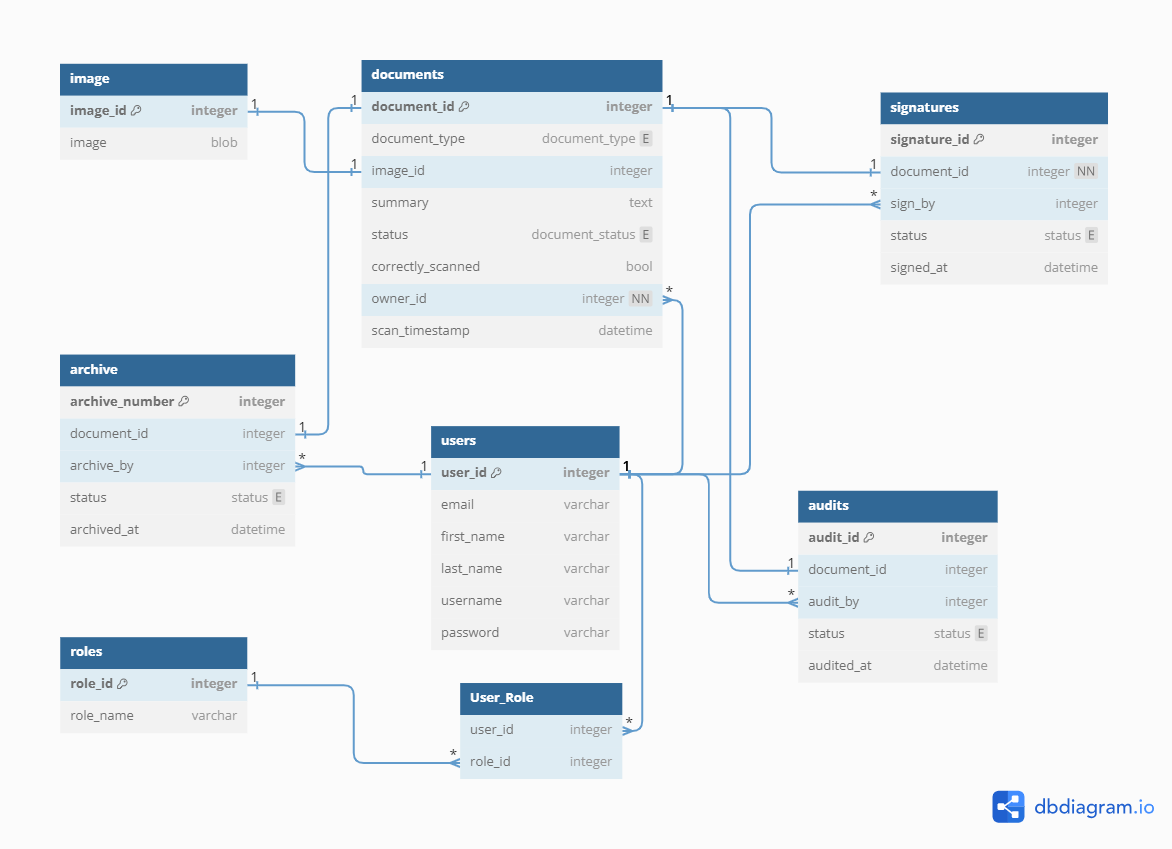
\includegraphics[width=\textwidth]{slike/dijagramBaze.PNG} 
					\caption{Dijagram baze podataka}
					\label{fig:dijagramBaze}
				\end{figure}
			
			\eject
			
			
		\section{Dijagram razreda}
		
			%\textit{Potrebno je priložiti dijagram razreda s pripadajućim opisom. Zbog preglednosti je moguće dijagram razlomiti na više njih, ali moraju biti grupirani prema sličnim razinama apstrakcije i srodnim funkcionalnostima.}\\
			
			%\textbf{\textit{dio 1. revizije}}\\
			
			%\textit{Prilikom prve predaje projekta, potrebno je priložiti potpuno razrađen dijagram razreda vezan uz \textbf{generičku funkcionalnost} sustava. Ostale funkcionalnosti trebaju biti idejno razrađene u dijagramu sa sljedećim komponentama: nazivi razreda, nazivi metoda i vrste pristupa metodama (npr. javni, zaštićeni), nazivi atributa razreda, veze i odnosi između razreda.}\\
			
			\begin{figure}[H]
				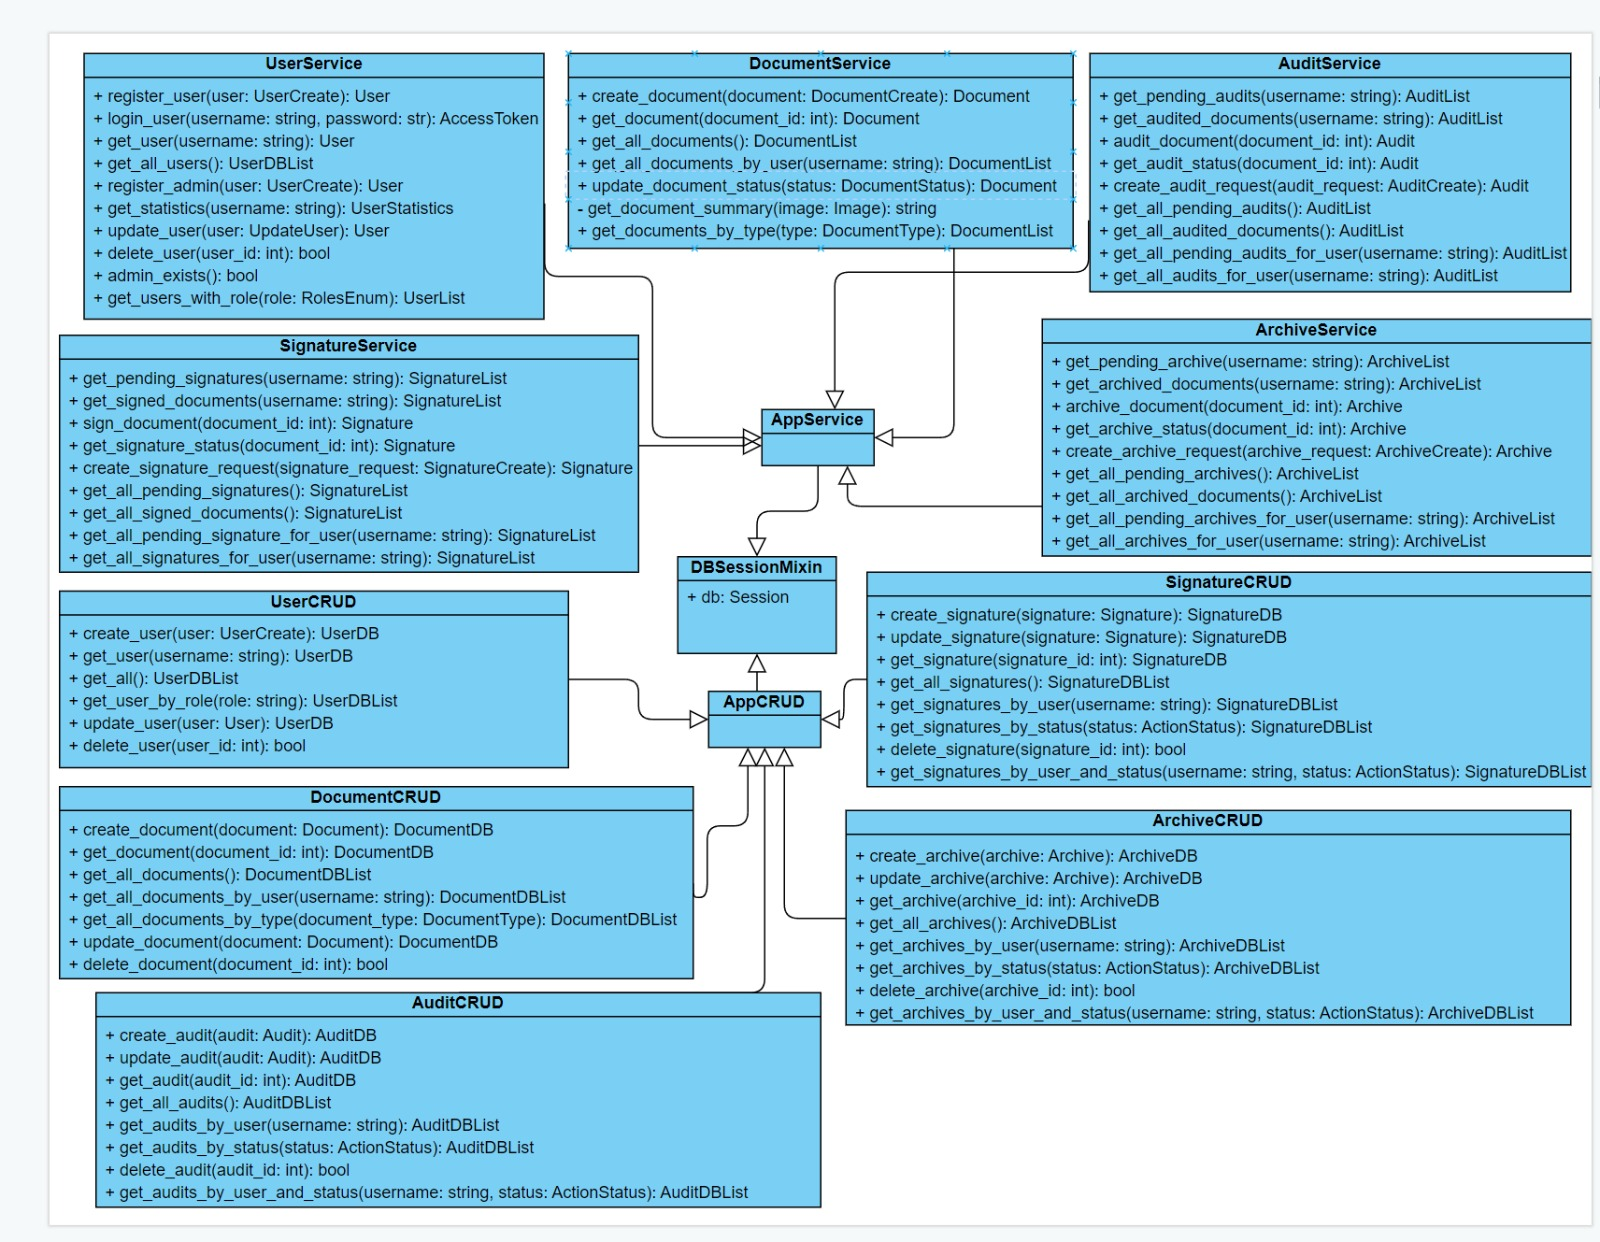
\includegraphics[width=\textwidth]{slike/razredi_serviceCRUD.jpg} 
				\caption{Dijagram razreda - servisi i CRUD}
				\label{fig:dijagramRazreda1}
			\end{figure}
			
			\begin{figure}[H]
				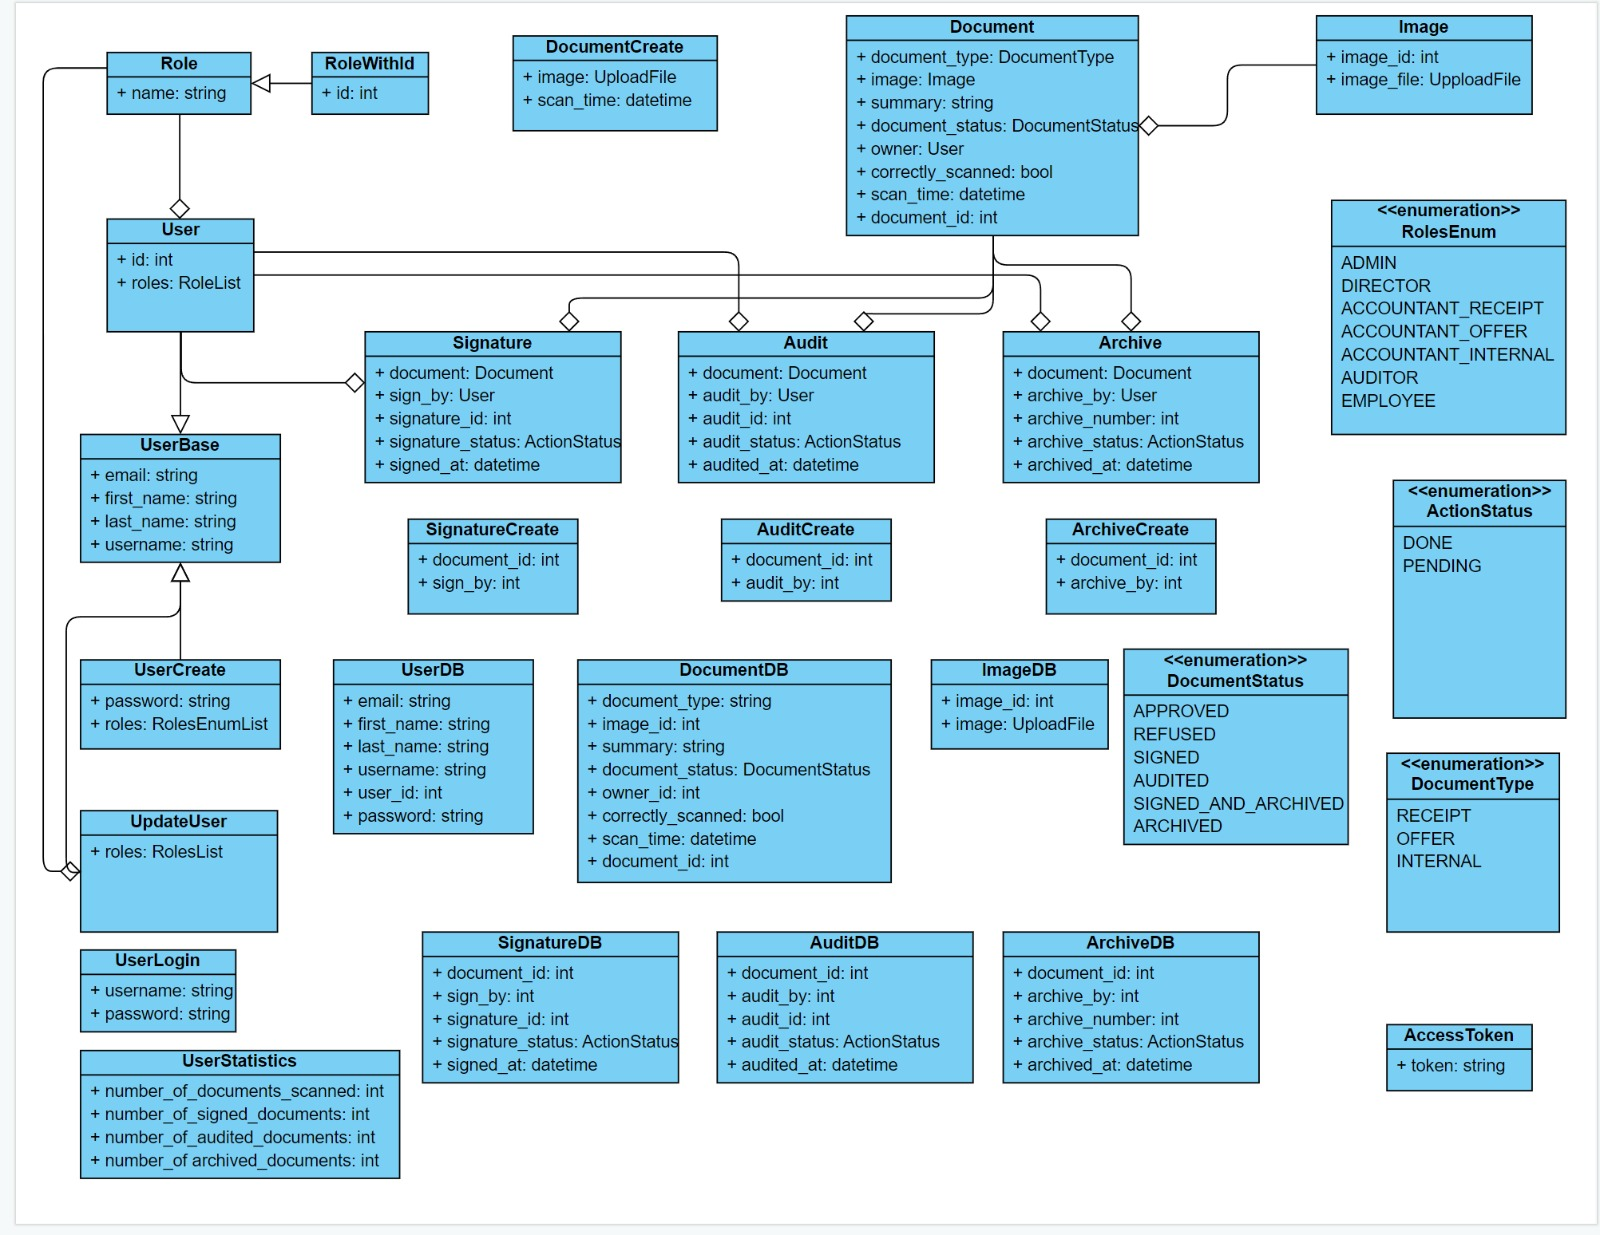
\includegraphics[width=\textwidth]{slike/razredi_shemaModel.jpg} 
				\caption{Dijagram razreda - shema i model}
				\label{fig:dijagramRazreda2}
			\end{figure}
			
			%\textbf{\textit{dio 2. revizije}}\\			
			
			%\textit{Prilikom druge predaje projekta dijagram razreda i opisi moraju odgovarati stvarnom stanju implementacije}
			
			
			
			\eject
		
		\section{Dijagram stanja}
			
			
			%\textbf{\textit{dio 2. revizije}}\\
			
			%\textit{Potrebno je priložiti dijagram stanja i opisati ga. Dovoljan je jedan dijagram stanja koji prikazuje \textbf{značajan dio funkcionalnosti} sustava. Na primjer, stanja korisničkog sučelja i tijek korištenja neke ključne funkcionalnosti jesu značajan dio sustava, a registracija i prijava nisu. }
			
			
			\eject 
		
		\section{Dijagram aktivnosti}
			
			%\textbf{\textit{dio 2. revizije}}\\
			
			 %\textit{Potrebno je priložiti dijagram aktivnosti s pripadajućim opisom. Dijagram aktivnosti treba prikazivati značajan dio sustava.}
			
			\eject
		\section{Dijagram komponenti}
		
			%\textbf{\textit{dio 2. revizije}}\\
		
			 %\textit{Potrebno je priložiti dijagram komponenti s pripadajućim opisom. Dijagram komponenti treba prikazivati strukturu cijele aplikacije.}